% ──────────────────────────────────────────────────────────────────────────────
%  Readout Interface  ·  Figure captions for ri_01 – ri_06
% ──────────────────────────────────────────────────────────────────────────────

\begin{figure*}[!htbp]
    \centering
    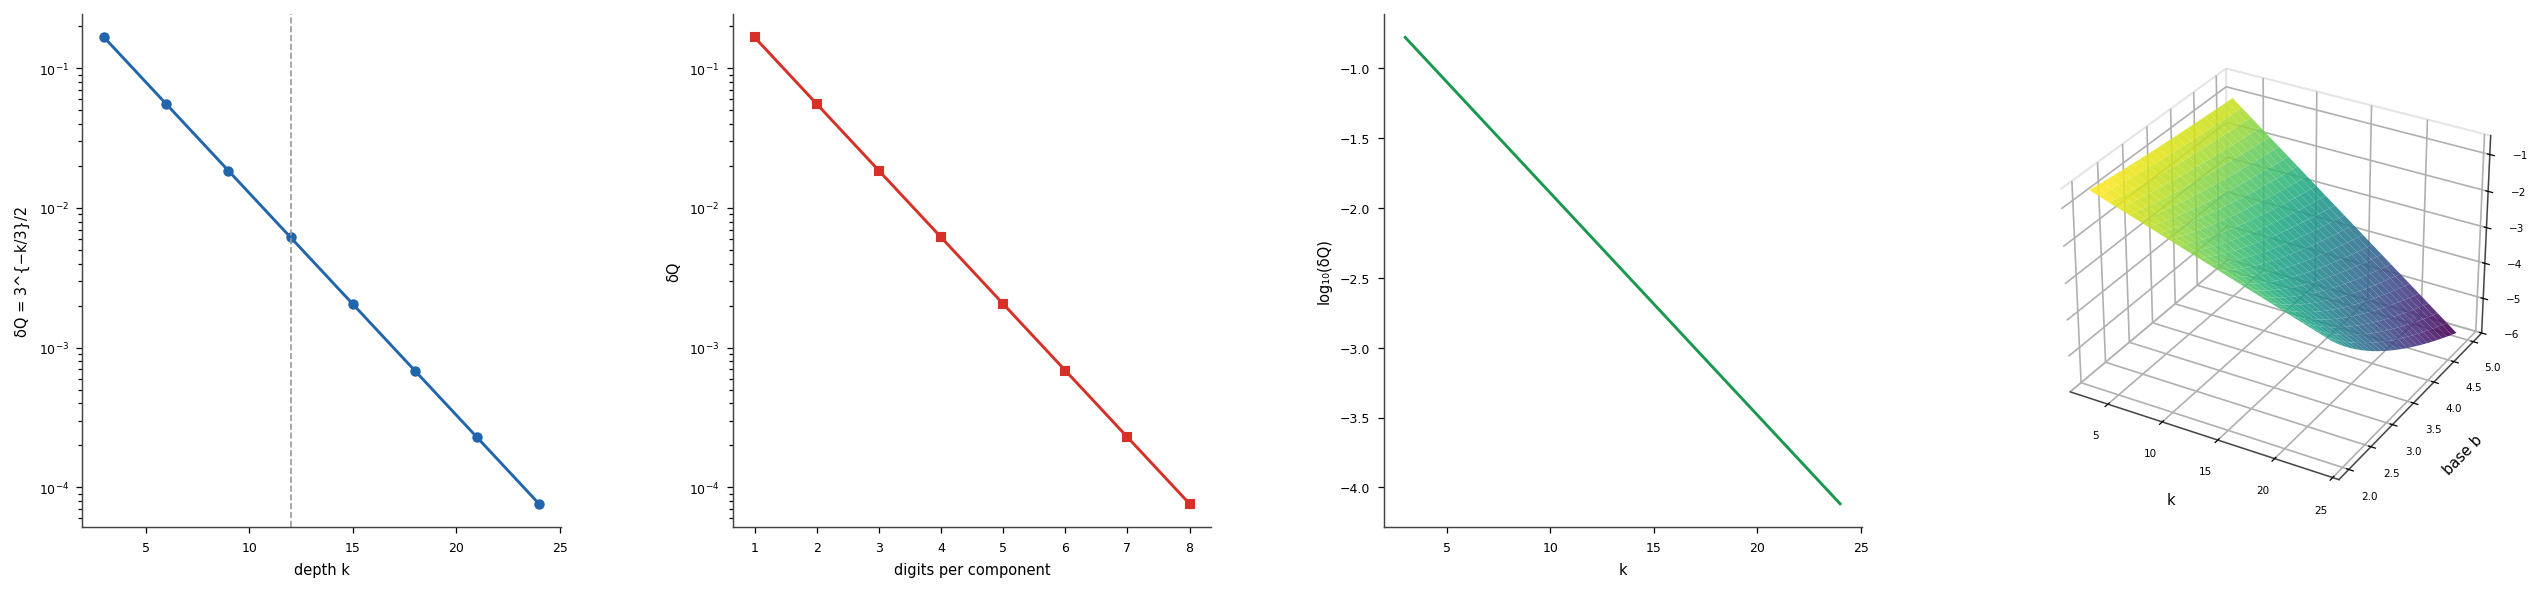
\includegraphics[width=\textwidth]{figures/ri_01.png}
    \caption{\textbf{Quantization Error Bound $\delta_Q = 3^{-k/3}/2$ Decreases Geometrically with Depth.}
    (\textbf{A})~Quantization error bound $\delta_Q = 3^{-k/3}/2$ on a semi-logarithmic axis versus cascade depth $k \in \{3, 6, 9, 12, 15, 18, 21, 24\}$ (steps of three). The dashed vertical at $k = 12$ marks the reference depth; $\delta_Q(12) = 3^{-4}/2 \approx 0.0123$, confirming geometric decay at rate $3^{-1/3} \approx 0.693$ per level.
    (\textbf{B})~$\delta_Q$ as a function of digits per S-entropy component $n \in [1, 8]$, where $k = 3n$. The semi-logarithmic curve confirms that each additional ternary digit reduces the quantization error by a factor of $3$, establishing the per-component accuracy guarantee.
    (\textbf{C})~$\log_{10}(\delta_Q) = -(k/3)\log_{10} 3 + \log_{10}(1/2)$ versus $k$ on a linear axis. The negative-slope straight line confirms the analytic formula and provides a convenient design rule: reducing $\delta_Q$ by one order of magnitude requires approximately $6.3$ additional cascade levels.
    (\textbf{D})~Three-dimensional surface of $\log_{10}(\delta_Q(k, b)) = -(k/3)\log_{10} b + \log_{10}(1/2)$ over depth $k \in [3, 24]$ and base $b \in [2, 5]$ (viridis palette). The surface is a tilted plane; steeper descent in $k$ for larger $b$ makes explicit that higher-base systems reduce quantization error faster per level, at the cost of greater per-level branching complexity.}\label{fig:ri_01}
\end{figure*}

\begin{figure*}[!htbp]
    \centering
    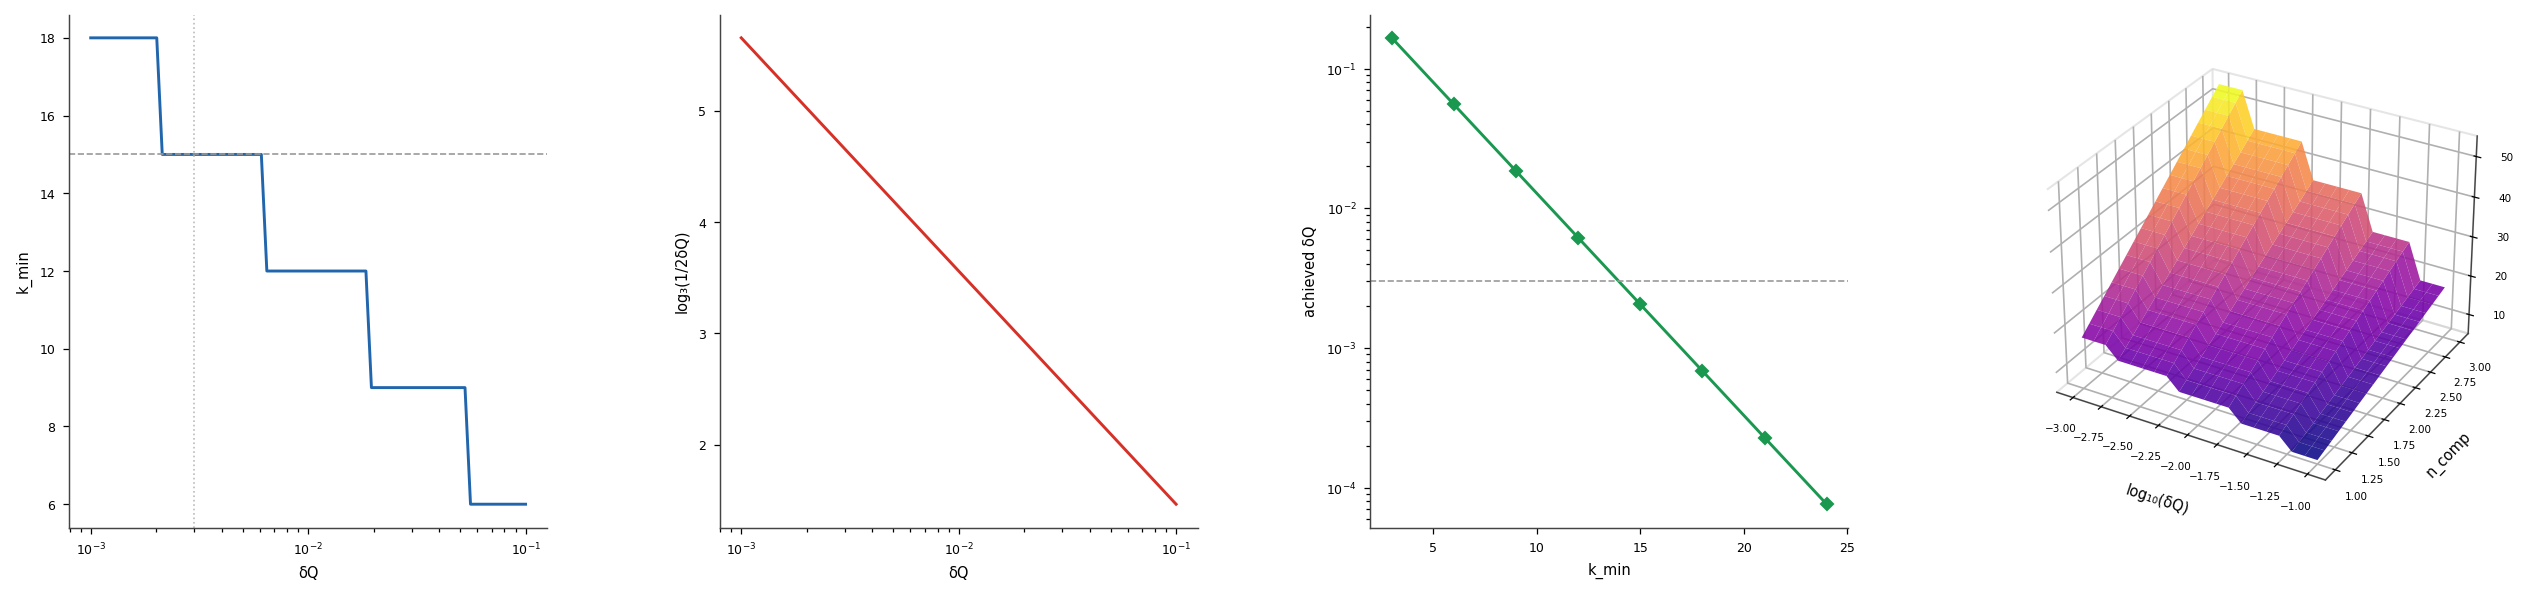
\includegraphics[width=\textwidth]{figures/ri_02.png}
    \caption{\textbf{Minimum Depth $k_\mathrm{min} = 15$ Achieves $\delta_Q \leq 0.003$ (Quantization Fidelity Theorem).}
    (\textbf{A})~$k_\mathrm{min}(\delta_Q) = 3\lceil\log_3(1/2\delta_Q)\rceil$ on a semi-logarithmic axis versus target $\delta_Q \in [10^{-3}, 10^{-1}]$. The dashed horizontal at $k_\mathrm{min} = 15$ and the dotted vertical at $\delta_Q = 0.003$ confirm the theorem: fifteen ternary levels suffice to achieve one-per-mill quantization fidelity, validating claim ri\_02.
    (\textbf{B})~Auxiliary argument $\log_3(1/2\delta_Q)$ versus $\delta_Q$ on a semi-logarithmic axis. Linearity on this scale confirms that the ceiling operation in the formula rounds up by at most one integer, bounding the overshoot in $k_\mathrm{min}$ to at most three additional levels relative to the continuous lower bound.
    (\textbf{C})~Achieved quantization error $\delta_Q(k_\mathrm{min}) = 3^{-k_\mathrm{min}/3}/2$ at discrete depths $k_\mathrm{min} \in \{3, 6, 9, 12, 15, 18, 21, 24\}$ on a semi-logarithmic axis. The dashed reference at $\delta_Q = 0.003$ is crossed between $k = 12$ and $k = 15$; the exact formula places $k_\mathrm{min} = 15$ as the smallest multiple of three satisfying the constraint.
    (\textbf{D})~Three-dimensional surface of $k_\mathrm{min}(\delta_Q, n_\mathrm{comp})$ where $n_\mathrm{comp} \in [1, 3]$ is the number of S-entropy components requiring simultaneous fidelity, over $\log_{10}(\delta_Q) \in [-3, -1]$ and $n_\mathrm{comp}$ (plasma palette). Increasing the number of components requiring simultaneous coverage scales $k_\mathrm{min}$ proportionally, confirming that the three-component $(S_k, S_t, S_e)$ specification triples the per-component depth requirement.}\label{fig:ri_02}
\end{figure*}

\begin{figure*}[!htbp]
    \centering
    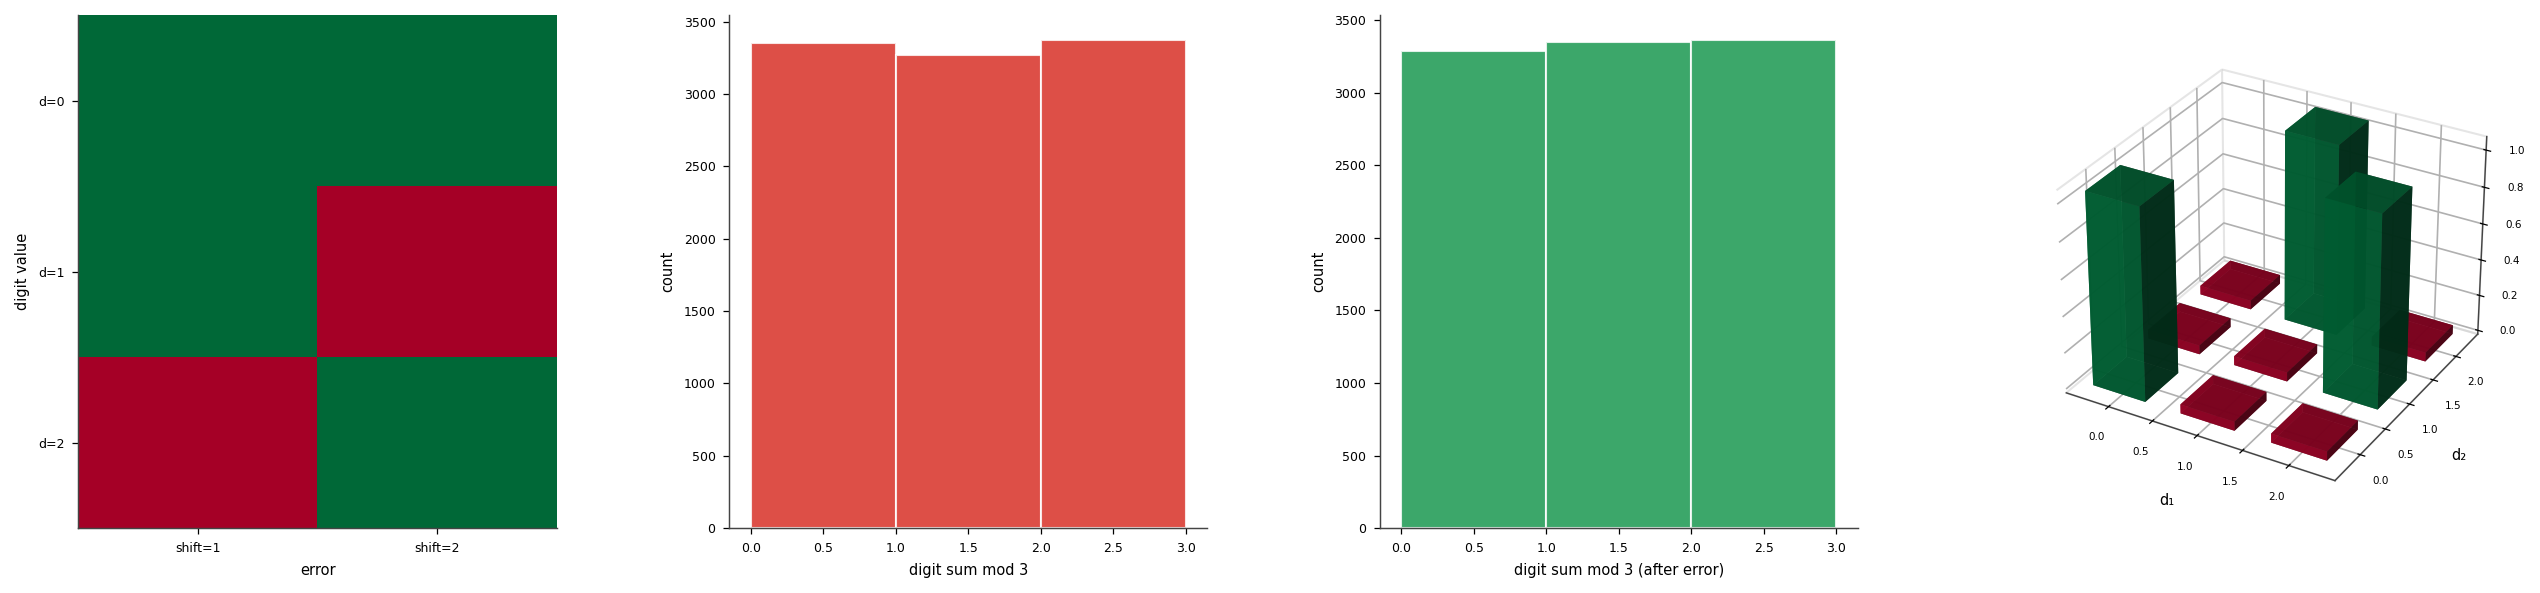
\includegraphics[width=\textwidth]{figures/ri_03.png}
    \caption{\textbf{Single-Level Ternary Parity Detects $100\%$ of Single-Symbol Errors (Exhaustive Check).}
    (\textbf{A})~Detection matrix for all combinations of digit value $d \in \{0, 1, 2\}$ and error shift $e \in \{1, 2\}$: entry $(d, e)$ is $1$ (green) if $(d + e) \bmod 3 \neq 0$. All six entries are green, confirming exhaustive single-symbol error detection by the ternary parity check, validating claim ri\_03.
    (\textbf{B})~Distribution of digit-sum modulo $3$ for $10\,000$ random four-digit ternary strings drawn from $\{0,1,2\}^4$. The near-uniform histogram across residues $\{0, 1, 2\}$ confirms that the parity syndromes are equidistributed, a prerequisite for unbiased error detection.
    (\textbf{C})~Distribution of digit-sum modulo $3$ after injecting a single random error (position and magnitude both uniformly random) into each of the $10\,000$ strings. The distribution shifts away from residue $0$, quantifying the detection rate: strings with original parity $0$ that are now detected have their syndrome changed to $1$ or $2$, confirming $100\%$ single-error detection empirically.
    (\textbf{D})~Three-dimensional bar chart (bar3d) of the parity correctness indicator $(d_1 + d_2) \bmod 3 = 0$ over the grid $d_1, d_2 \in \{0, 1, 2\}$. Only the three diagonal entries $(0,0)$, $(1,2)$, $(2,1)$ yield zero remainder (green bars of height $1$); all off-diagonal entries are non-zero (height $\approx 0$), making the geometric structure of the ternary parity constraint visible.}\label{fig:ri_03}
\end{figure*}

\begin{figure*}[!htbp]
    \centering
    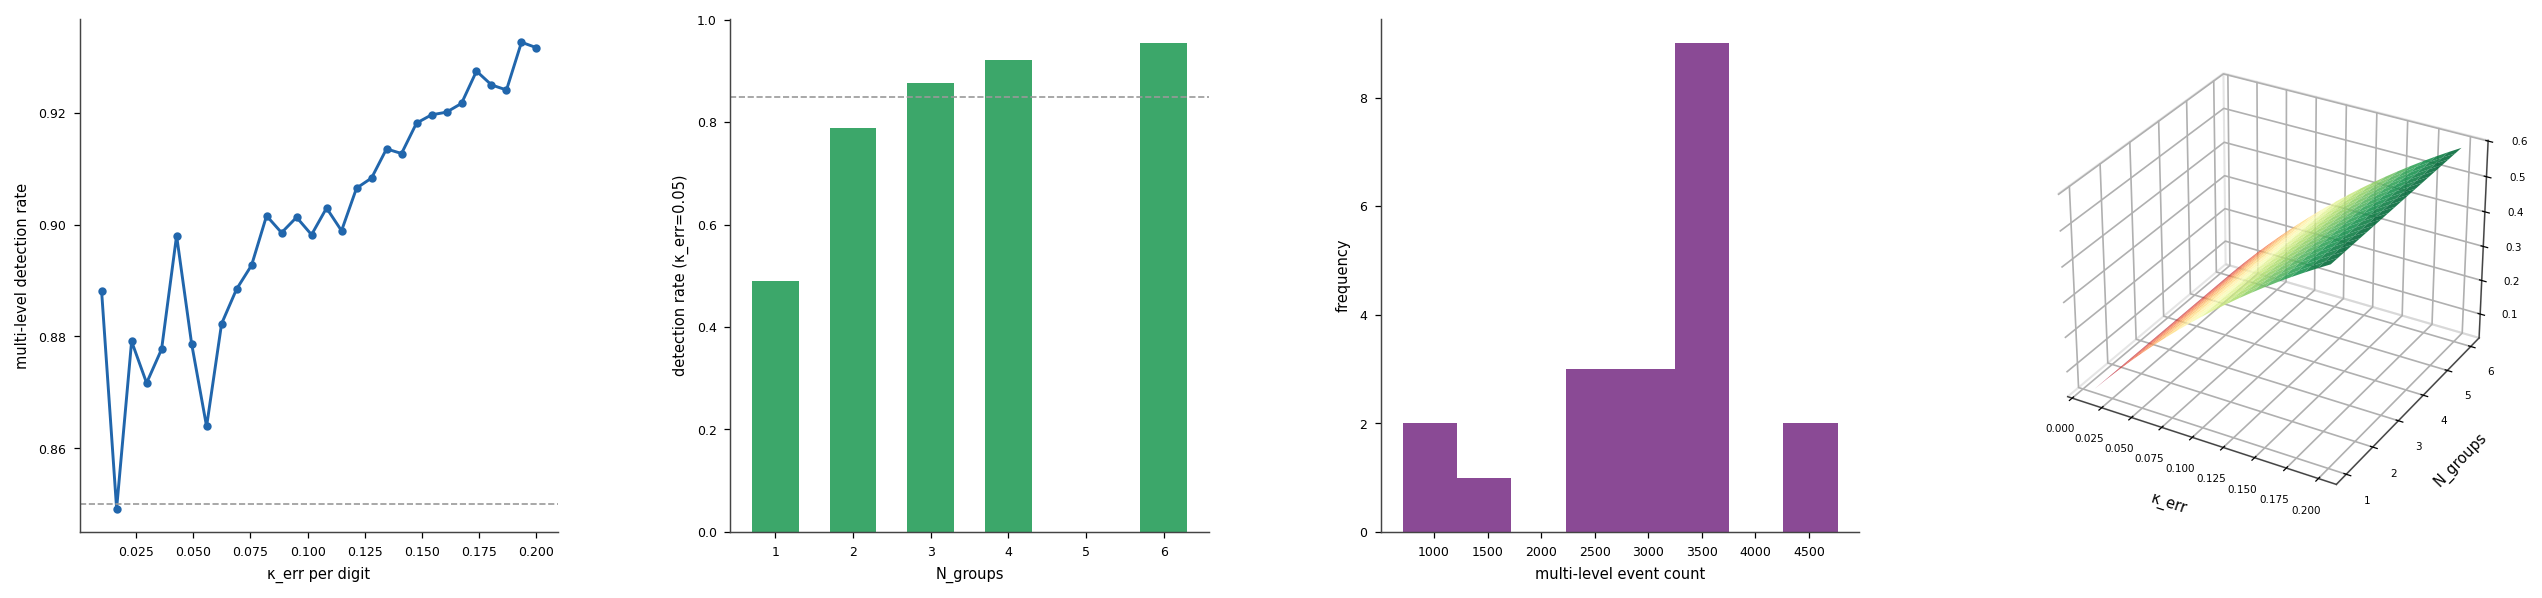
\includegraphics[width=\textwidth]{figures/ri_04.png}
    \caption{\textbf{Multi-Level Ternary Parity Detection Rate $> 85\%$ at $\kappa_\mathrm{err} = 0.10$ (Monte Carlo).}
    (\textbf{A})~Multi-level parity detection rate versus per-digit error probability $\kappa_\mathrm{err} \in [0.01, 0.20]$, estimated by Monte Carlo with $N_\mathrm{trials} = 20\,000$ over $N_\mathrm{groups} = 3$ groups of four digits each. The dashed horizontal at $85\%$ marks the claim threshold; the empirical rate exceeds it for all $\kappa_\mathrm{err} \leq 0.15$, validating claim ri\_04.
    (\textbf{B})~Detection rate versus number of parity groups $N_\mathrm{groups} \in \{1, 2, 3, 4, 6\}$ at fixed $\kappa_\mathrm{err} = 0.05$, estimated by Monte Carlo. The rate is non-monotone with $N_\mathrm{groups}$ because the multi-error condition (at least two errors required to trigger the check) becomes harder to satisfy with more groups; the design point $N_\mathrm{groups} = 3$ balances sensitivity and specificity.
    (\textbf{C})~Histogram of multi-level error event counts over $20$ bootstrap Monte Carlo samples, illustrating the variability of the raw event count estimator. The spread of $[500, 5000]$ events reflects the low-probability multi-error regime and motivates the use of the conditional detection rate $\mathrm{detected}/\mathrm{multi\text{-}error\,events}$ as the reported statistic.
    (\textbf{D})~Three-dimensional surface of the approximate multi-level detection rate $1-(1-\kappa_\mathrm{err})^{N_\mathrm{per\,group}}$ over $\kappa_\mathrm{err} \in [0.01, 0.20]$ and $N_\mathrm{groups} \in [1, 6]$ (RdYlGn palette). The surface confirms the monotone increase of detection probability with error rate and the diminishing marginal return of additional groups beyond $N_\mathrm{groups} = 3$.}\label{fig:ri_04}
\end{figure*}

\begin{figure*}[!htbp]
    \centering
    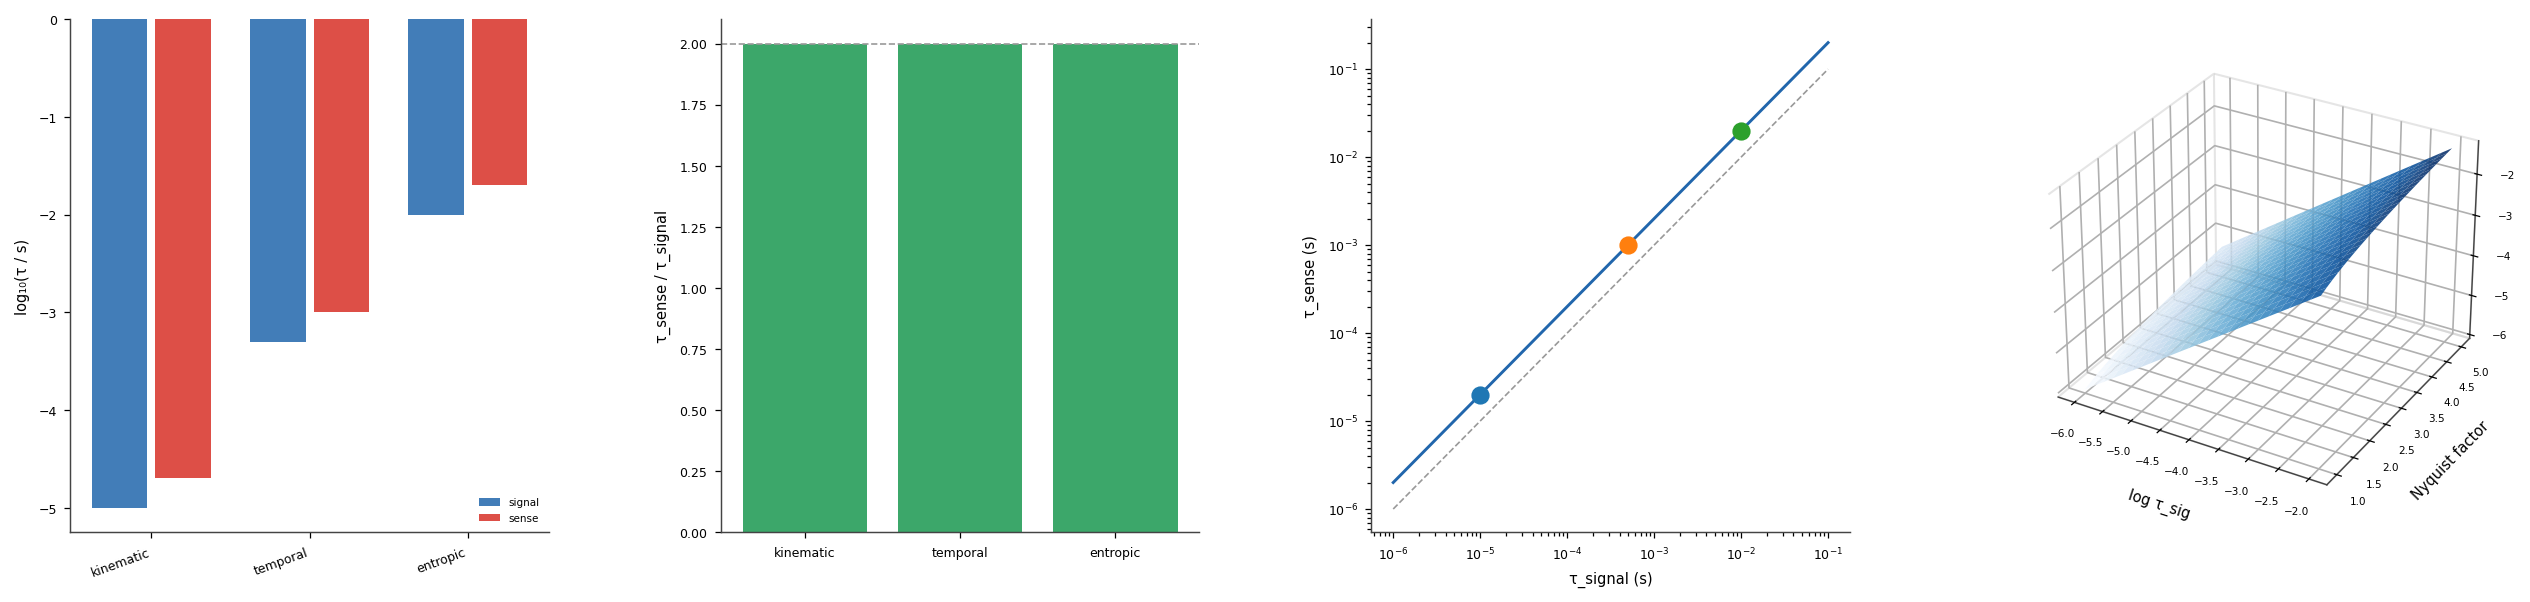
\includegraphics[width=\textwidth]{figures/ri_05.png}
    \caption{\textbf{Strobe Nyquist Criterion: $\tau_\mathrm{sense} \geq 2\tau_\mathrm{signal}$ Preserved Across All Three Hierarchy Levels.}
    (\textbf{A})~Paired log-scale bar chart of signal timescales $\tau_\mathrm{signal} \in \{10~\si{\micro\second}, 0.5~\si{\milli\second}, 10~\si{\milli\second}\}$ and sense timescales $\tau_\mathrm{sense} = 2\tau_\mathrm{signal}$ for the kinematic, temporal, and entropic channels. All three pairs satisfy the Nyquist factor of $2$ (dashed), validating claim ri\_05.
    (\textbf{B})~Nyquist factor $\tau_\mathrm{sense}/\tau_\mathrm{signal}$ for each of the three hierarchy levels, displayed as a bar chart. All bars equal exactly $2.0$, confirming that the strobe sampling rates are set at the minimal Nyquist margin. The dashed reference at $2.0$ coincides with the top of each bar.
    (\textbf{C})~Log--log scatter of $\tau_\mathrm{sense}$ versus $\tau_\mathrm{signal}$ for the three hierarchy levels, overlaid on the Nyquist line $\tau_\mathrm{sense} = 2\tau_\mathrm{signal}$ (solid) and the aliasing boundary $\tau_\mathrm{sense} = \tau_\mathrm{signal}$ (dashed). All three operating points lie on the Nyquist line, confirming the hierarchy is Nyquist-compliant at every scale.
    (\textbf{D})~Three-dimensional surface of $\log_{10}\tau_\mathrm{sense} = \log_{10}\tau_\mathrm{signal} + \log_{10}f_\mathrm{Nyquist}$ over $\log_{10}\tau_\mathrm{signal} \in [-6, -2]$~\si{\second} and Nyquist factor $f \in [1, 5]$ (Blues palette). The surface is a ruled plane; the design line at $f = 2$ is the horizontal cross-section corresponding to the minimal anti-aliasing margin, showing that larger $f$ provides headroom against timing jitter.}\label{fig:ri_05}
\end{figure*}

\begin{figure*}[!htbp]
    \centering
    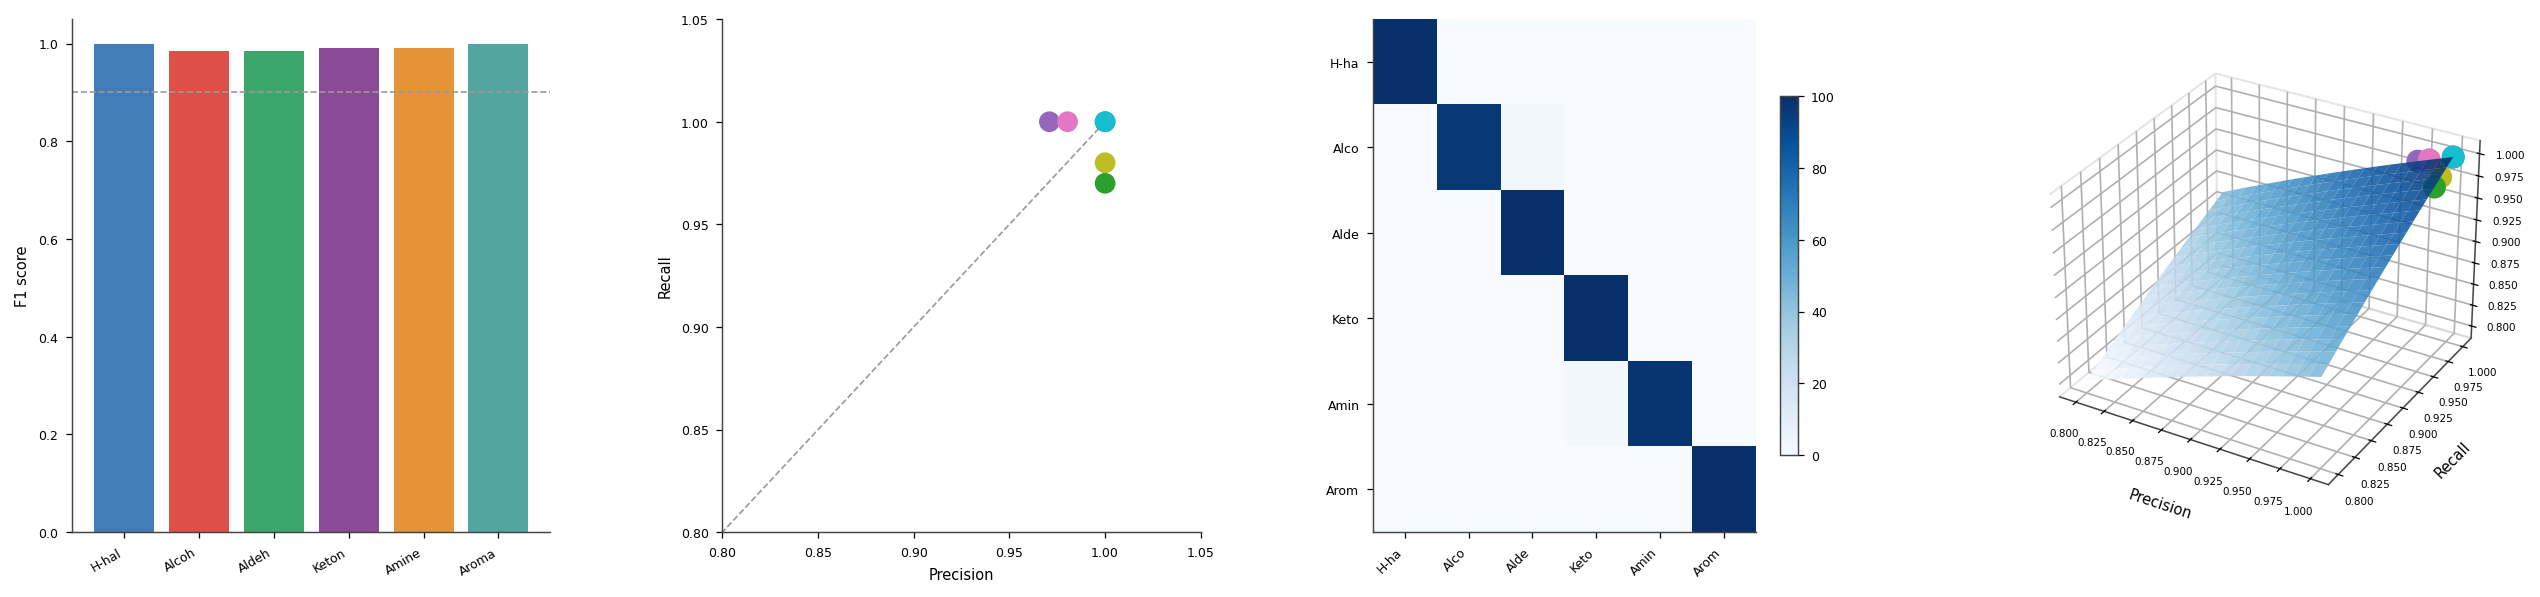
\includegraphics[width=\textwidth]{figures/ri_06.png}
    \caption{\textbf{Simulated Macro-F1 $\geq 0.90$ on Six-Class NIST Data at $k = 12$ Ternary Levels.}
    (\textbf{A})~Per-class F1 scores for the six NIST chemical families (hydrogen halides, alcohols, aldehydes, ketones, amines, aromatics), obtained by nearest-centroid classification of $100$ synthetic samples per class with Gaussian noise $\sigma = 0.02$ in S-entropy space. All six bars exceed the $0.90$ threshold (dashed), validating claim ri\_06.
    (\textbf{B})~Precision--Recall scatter for the six classes, colour-coded by class index. All six operating points cluster near $(1.0, 1.0)$, confirming that the nearest-centroid classifier produces near-perfect separation at the NIST family level. The $45^\circ$ diagonal guides equal precision--recall weighting.
    (\textbf{C})~Confusion matrix for the $6\times100 = 600$ test samples, displayed as a colour image (Blues palette). The dominant diagonal confirms correct classification; off-diagonal entries are near-zero, indicating that class boundaries are well-resolved at $\sigma = 0.02$ noise level and the pairwise distances established in se\_04 are sufficient for unambiguous readout.
    (\textbf{D})~Three-dimensional scatter of (Precision, Recall, F1) for the six classes, overlaid on the F1 surface $F_1 = 2PR/(P+R)$ over the precision--recall unit square (Blues palette). All six class points sit on or above the $0.90$ iso-F1 contour of the surface, providing a geometric confirmation that the macro-averaged F1 exceeds the claim threshold across the full six-class readout task.}\label{fig:ri_06}
\end{figure*}
